\chapter{Data Origin Authentication in the Quantum Networking Stack}
\label{chp:doa}

\begin{abstract}
Typically, quantum networking protocols make use of classical communications to coordinate
entanglement generation and other tasks. In this chapter, we discuss the need for authentication of
such classical messages exchanged at the quantum network stack level, with focus on concrete
protocol proposals. We then experimentally measure the overhead incurred by sending authenticated
classical messages through an authentication system that uses key material supplied by an
\acrshort{mdiqkd} system. We use this information to simulate the performance of a quantum link
whose protocol stack uses an authenticated classical channel, and compare that to existing
simulations of the same protocol stack. We find that message authentication overhead is not
detrimental to entanglement requests that end with an immediate measurement of the qubit, but has a
much more pronounced effect on entanglement requests that require storing the entangled qubit in
memory, and thus must be carried out sequentially.
\end{abstract}

\noindent
\note{This chapter is extracted from the data origin authentication paper. There aren't any major
additions.}

\blfootnote{
    This chapter is based on the preprint: \fullcite{abrahams_2023_doa_noprint}. \note{Add proper
    link to arXiv when submitted}
}

\newpage

\lettrine{U}{p} until now, several proposals have been put forward as to how quantum networks should
be structured~\cite{van_meter_2013_repeaters, schoute_2016_shortcuts, joshi_2020_trusted}.
Researchers are also investigating how to abstract the complex physics of quantum networking so as
to provide platform-independent services to the end user~\cite{dahlberg_2019_egp,
pirker_2019_quantum, illiano_2022_quantum} --- the most basic of services being \emph{entanglement
generation}. One proposal for a \emph{quantum network stack} provides an outline of the layers and
separation of responsibilities, as well as protocols to populate these
layers~\cite{dahlberg_2019_egp, kozlowski_2020_qnp}. Within the proposed stack, each layer makes use
of the service exposed by the layer below, and provides a higher-level service to the layer
above~\cite{dahlberg_2019_egp}. This stack is inspired by the well-known \acrshort{tcpip} stack for
classical networks, and is illustrated in \cref{fig:functional-allocation}. Each protocol within the
quantum network stack makes use of classical control messages, exchanged over a classical network,
to coordinate quantum communication activities. These messages together form what we refer to as the
\emph{classical data plane} --- which lives alongside the \emph{quantum data plane}, where
information encoded in the quantum system is transmitted.

\begin{figure}[b]
    \centering
    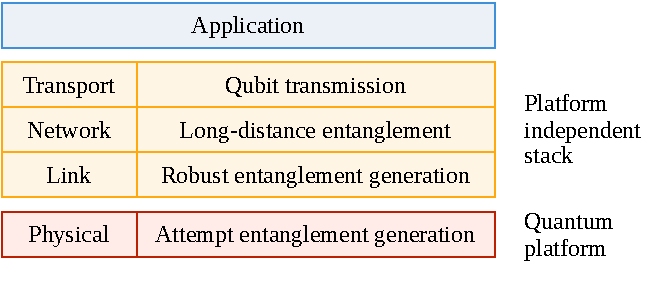
\includegraphics[width=0.6\linewidth]{figures/functional-allocation.pdf}
    \caption{
        Functional allocation of layers in a quantum network stack, adapted from
        Ref.~\cite{dahlberg_2019_egp}. The physical layer is quantum platform-dependent. The link
        layer provides platform-independent robust entanglement generation. All subsequent layers
        are therefore also platform independent, including the network and optionally transport
        layers which facilitate end-to-end entanglement between non-adjacent nodes. The application
        layer uses the services offered by the stack to perform quantum networking tasks.
    }
    \label{fig:functional-allocation}
\end{figure}

Such classical messages must be transmitted in a secure manner for a quantum network to function
reliably. \citeauthor{satoh_2020_attacking} mention forged classical messages as a general concern
for quantum networks~\cite{satoh_2020_attacking}. To prevent such forgeries, quantum network nodes
may employ \acrfull{doa}, to distinguish between genuine and fraudulent classical messages.
\acrshort{doa} is performed using a secret which is shared between two parties. A \acrfull{mac}
produces a tag for each message both at the sending and at the receiving end, to verify that the
message contents
%
\begin{inlinelist}
    \item were not altered and
    \item were produced by a party which owns the shared secret.
\end{inlinelist}
%
This structure is illustrated in \cref{fig:mac-structure}.

\begin{figure}[t]
    \centering
    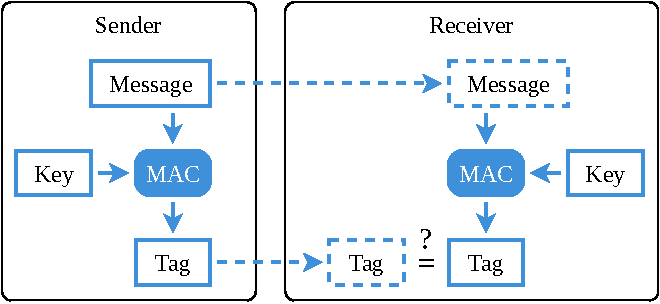
\includegraphics[width=0.6\linewidth]{figures/mac-structure.pdf}
    \caption{
        General structure of a \acrfull{mac}, where sender and receiver have a shared key. The
        receiver checks the output of the \acrshort{mac} to verify that the message was not modified
        in transit.
    }
    \label{fig:mac-structure}
\end{figure}

When designing control protocols for quantum networks, one should carefully estimate their impact on
end-to-end entanglement generation latency. Besides the more obvious reasons to do so, there is a
fundamental aspect of quantum information that imposes strict constraints on end-to-end latency:
storing quantum data reliably for extended periods of time is non-trivial. Qubits have relatively
short lifetimes, usually of the order of milliseconds, or at best of a few
seconds~\cite{abobeih_2018_one_sec, bradley_2019_one_min}. Therefore, not only can high end-to-end
latency affect the quality of the service offered by the network, but in some cases it may result in
no service at all. Classical processing and communication overhead must, thus, be kept to a minimum,
such that the entangled qubits can be used as quickly as possible.

Inevitably, performing \acrshort{doa} on messages exchanged in the classical data plane would incur
some computation and communication overhead. Such overhead is typically neglected when modeling,
simulating, or experimentally validating network protocols for quantum communications. In this work,
we illustrate the effects of classical authentication on a hypothetical quantum link. We first
experimentally measure the delays incurred by \acrshort{doa}, when performed on a sample of
classical messages using a \acrshort{qkd}-powered authentication proxy. We then analyze the behavior
of the hypothetical quantum link --- using a simulator for quantum
networks~\cite{coopmans_2021_netsquid} --- where the model of the classical communication channel of
such setup includes the measured classical delays incurred by \acrshort{doa}. The contributions of
this work are as follows:

\begin{enumerate}
    \item We provide a concise motivation for why \acrshort{doa} is a necessary component to uphold
          the availability of system-level protocols of the quantum network stack, and to help
          maintain the integrity of quantum data.
    \item We experimentally measure the delays incurred by \acrshort{doa}, performed using a
          \acrshort{qkd}-based authentication system, when run on a classical communication link.
    \item We offer a quantitative analysis of the impact of \acrshort{doa}, using the delays
          measured as per the previous point, when applied to the quantum network protocols of a
          hypothetical quantum link, as introduced in Ref.~\cite{dahlberg_2019_egp}.
\end{enumerate}

\section{Related Work}
\label{sec:doa:relwork}

Classical networking is an essential component of quantum networks and quantum networking
applications. \citeauthor{kozlowski_2019_towards} mention that the security of classical
communications is of concern when designing a quantum network~\cite{kozlowski_2019_towards}.
\citeauthor{satoh_2020_attacking} present a general motivation for authenticating the classical
channel of a quantum link~\cite{satoh_2020_attacking}. They model attack vectors on quantum
communications through the lens of \acrfull{cia}. Without any security measures in place, an
attacker may:

\begin{itemize}
    \item Disrupt the network in any number of ways, affecting its \emph{availability}.
    \item Interfere with data sent via the network, hampering the \emph{integrity} of quantum data.
    \item Read quantum data through the accompanying classical data, affecting
          \emph{confidentiality}.
\end{itemize}
Even though the confidentiality of quantum data itself is solely the responsibility of the
application layer (\cref{fig:functional-allocation}), privacy concerns such as \emph{tracking} are
still an issue if an attacker can read all classical communication.

All proposals of quantum network designs and quantum network protocols identified use some form of
classical communication to coordinate quantum communication and
entanglement~\cite{van_meter_2013_repeaters, schoute_2016_shortcuts, joshi_2020_trusted,
pirker_2019_quantum, kozlowski_2019_towards, dahlberg_2019_egp, kozlowski_2020_qnp}. We investigate
one such proposal for a quantum network stack, the one put forth by \textcite{dahlberg_2019_egp},
which has been evaluated in simulation, as well as on hardware~\cite{pompili_2022_experimental}
(\cref{chp:netstack}), and extended by \textcite{kozlowski_2020_qnp}.

The proposed protocol stack for quantum networks includes physical, link, network, transport, and
application layers, as illustrated in \cref{fig:functional-allocation}. The physical layer protocol,
called \acrfull{mhp}~\cite{dahlberg_2019_egp}, performs heralded entanglement generation attempts,
replying using a single repeater station. At the link layer, the
\acrfull{qegp}~\cite{dahlberg_2019_egp} has an internal retry mechanism and performs coordination
between adjacent nodes to provide more robust entanglement generation. \acrshort{qegp} accepts two
types of requests from the layer above:
%
\begin{inlinelist}
    \item \acrlong{ck} (\acrshort{ck}), to create an entangled pair and store it in memory;
    \item \acrlong{md} (\acrshort{md}), to create entangled pair, measure it, and report is outcome.
\end{inlinelist}
At the network layer, the \acrfull{qnp}~\cite{kozlowski_2020_qnp} coordinates entanglement
generation and swap operations on the full chain of intermediate nodes between two non-adjacent end
nodes.

We analyze the three service-level protocols \acrshort{mhp}, \acrshort{qegp}, and \acrshort{qnp},
and illustrate why \acrfull{doa} is important for these protocols to function, mostly with regards
to \emph{availability} of the network, and \emph{integrity} of quantum data.

\section{Why Data Origin Authentication}
\label{sec:doa:why}

We investigate the applicability of \acrlong{doa} to three system-level protocols for quantum
network stacks: \acrshort{mhp}, \acrshort{qegp} and \acrshort{qnp}~\cite{dahlberg_2019_egp,
kozlowski_2020_qnp}. Quantum application protocols (e.g. \acrshort{qkd}) lie outside the scope of
this work. Here, we provide a non-exhaustive list of example actions that a malicious actor may
perform if they are allowed to forge or modify classical messages exchanged at the protocol level.
We mention whether each action affects the \emph{availability} of the link or network, or the
\emph{integrity} of the quantum data sent via the network.

\paragraph{Physical layer}

\acrshort{mhp} operates at the physical layer. Hardware vulnerabilities of the physical entanglement
generation process are outside the scope of this work.

\begin{example}
\textit{Availability.}
Change a successful heralding signal to an error code such Alice and Bob falsely conclude that
entanglement has failed.
\end{example}

\begin{example}
\textit{Integrity.}
Modify the heralding signal from the midpoint station by changing the state announcement such that
Alice or Bob apply the wrong Pauli corrections to their qubits.
\end{example}

\begin{example}
\textit{Integrity.}
Interfere with mismatch verification~\cite{dahlberg_2019_egp, pompili_2022_experimental} such that
Alice and Bob falsely conclude that a \acrshort{mhp} request belongs to the same \acrshort{qegp}
request, thus hampering the integrity of quantum data due to cross-process interference.
\end{example}

\paragraph{Link layer}

\acrshort{qegp} operates at the link layer~\cite{dahlberg_2019_egp}. As proposed in
Ref.~\cite{dahlberg_2019_egp}, it is used to synchronize entanglement requests, and to communicate
the number of available memory qubits and the expiration of requests.

\begin{example}
\textit{Availability.}
Continually send requests for entanglement, exhausting the resources of nodes receiving
them~\cite{kozlowski_2019_towards}.
\end{example}

\begin{example}
\textit{Availability.}
When advertising the number of available communication or storage qubits, set either to 0. The
receiving node then assumes that there are no communication or storage qubits available on the
sending node.
\end{example}

\begin{example}
\textit{Integrity.}
Change the qubit identifier of an entanglement generation request such that Alice and Bob entangle
the wrong data qubits, causing cross-path or process interference.
\end{example}

\paragraph{Network layer}

\acrshort{qnp} operates at the network layer. Conceptually, it allows non-adjacent nodes in a
quantum network to coordinate entanglement generation. This is akin to the \acrfull{ip} in the
classical stack. It makes use of \texttt{FORWARD} and \texttt{TRACK} messages to track entanglement
generation~\cite[Figure 6]{kozlowski_2020_qnp}. \texttt{FORWARD} messages are used to communicate
entanglement requests, and \texttt{TRACK} messages contain classical correction information for both
end-nodes in the network.

\begin{example}
\textit{Availability.}
Modify \texttt{FORWARD} message so that intermediary nodes do not receive entanglement swap
instructions.
\end{example}

\begin{example}
\textit{Integrity.}
Modify \texttt{TRACK} messages such that the end-nodes of a path do not receive the correct
entanglement swap outcome, and thus apply the wrong corrections to their qubits.
\end{example}

\begin{figure}[t]
    \centering
    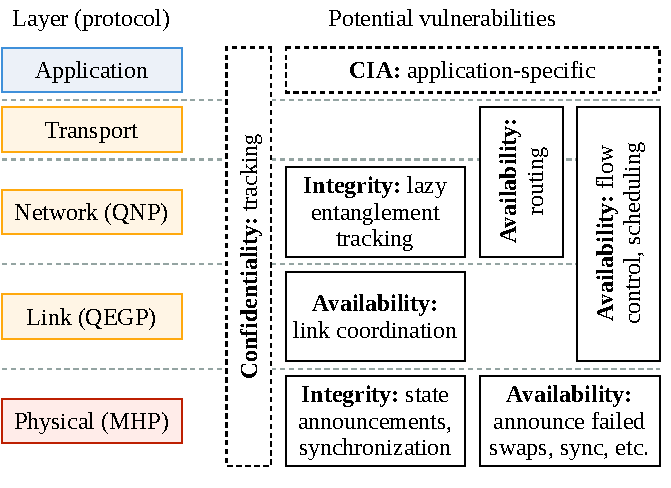
\includegraphics[width=0.6\linewidth]{figures/doa-examples.pdf}
    \caption{
        Example effects of tampering with control messages at each layer of the quantum network
        stack through the lens of \acrfull{cia}. We take as examples concrete implementations of
        quantum network protocols --- including \acrshort{qnp}, \acrshort{qegp} and
        \acrshort{mhp}~\cite{kozlowski_2020_qnp, dahlberg_2019_egp} --- to highlight the potential
        vulnerabilities at each layer. In this work, we do not focus on confidentiality issues (see
        Ref.~\cite{satoh_2020_attacking}).
    }
    \label{fig:doa-examples}
\end{figure}

We illustrate the concerns of availability and data integrity in a quantum network stack in
\cref{fig:doa-examples}. Such security threats are addressed in part by using \acrlong{doa}, which
can prevent modification and forgery of classical control messages. It should be noted, however,
that availability may still be hampered by an adversary capable of halting transmission of classical
control messages outright. Furthermore, if a malicious actor were to gain access to a node itself
then this might circumvent many or all security mechanisms in place, including \acrshort{doa}, and
should therefore also be prevented.

More in general, we also note that classical control messages might reveal information about who is
using the network and the types of operations being performed. Therefore, in a more mature network,
it will likely be worthwhile to also encrypt the contents of control messages.
\citeauthor{satoh_2020_attacking} mention tracking as a general concern for inter-node classical
communication within the quantum stack~\cite{satoh_2020_attacking}. Encryption combined with
transmission of random noise could address tracking concerns.

\section{Experimental Methodology}
\label{sec:doa:meth}

We aim to illustrate the effects of \acrlong{doa}, and the total overhead incurred by classical
control messages, on the performance of a hypothetical quantum link. To limit the scope of our
investigation, we focus on the performance of link and physical layer protocols as proposed by
\textcite{dahlberg_2019_egp}, and we extend the simulation therein such that it fully models
%
\begin{inlinelist}
    \item classical transmission overhead and
    \item \acrshort{doa} overhead.
\end{inlinelist}

Instead of modeling communication overhead analytically, we measure it experimentally by recording
\acrfull{rtt} of sample control messages sent and authenticated through a full-blown data
authentication proxy. The proxy tags classical messages using key material obtained from a
\acrfull{mdiqkd} key server, based on the work by \textcite{berrevoets_2022_deployed}. We then
inject the measured overhead into the simulation parameters, and then extract performance metrics as
done in Ref.~\cite{dahlberg_2019_egp}. The process of measuring classical communication overhead is
explained in \cref{sec:doa:latency}, while the simulation results are presented in
\cref{sec:doa:results}.

\section{Measuring Classical Latency}
\label{sec:doa:latency}

In order to obtain an estimate of the expected latency incurred by classical control messages in a
quantum network stack, we measure the \acrfull{rtt} of a sample of messages when sent through an
authenticated classical channel in the field. The messages are \acrshort{icmp} (ping) packets, sized
to mimic \acrshort{qegp} and \acrshort{mhp} packets. The authentication mechanism is external to the
nodes exchanging ping messages, acting as a proxy between them. The proxy's \acrshort{mac}
calculates a tag over the sent message, transmits the message and the tag, and verifies the tag at
the receiving end before delivering the message to the destination node. The experimental setup is
depicted in \cref{fig:mac-setup-diagram}.

Ping messages are exchanged between two real-time classical network nodes similar to those used in
the experimental validation of \acrshort{qegp}~\cite{pompili_2022_experimental}
(\cref{chp:netstack, chp:qnodeos}) --- MicroZed boards~\cite{microzed} running a
FreeRTOS~\cite{freertos} application --- connected to the proxy via a Gigabit Ethernet interface.
The source node records the \acrshort{rtt} of the message, and computes various statistics on these
timestamps, most notably average and standard deviation. We use these statistics to extrapolate the
expected classical communication latency for the various simulation scenarios presented in
\cref{sec:doa:results}.

The \acrfull{mac} on both ends retrieves authentication keys from a local key server, which contains
key material identical to its counterpart at the other end. Key material is produced by an
\acrshort{mdiqkd} implementation deployed in the Utrecht area, in the Netherlands. The
\acrshort{mdiqkd} system is very similar to the one implemented in
Ref.~\cite{berrevoets_2022_deployed}, though with a few differences. Firstly, the upgraded system
uses a four-intensity decoy state protocol~\cite{zhou_2016_making, woodward_2021_gigahertz}, which
improves key rate. This is an improvement over the three-intensity decoy state
protocol~\cite{yu_2013_three} of the previous deployment. Second, there are now separate, dedicated
fiber-optic cables for quantum and classical messages. In the original system these were combined,
at the cost of reduced key rate.

\begin{figure}[t]
    \centering
    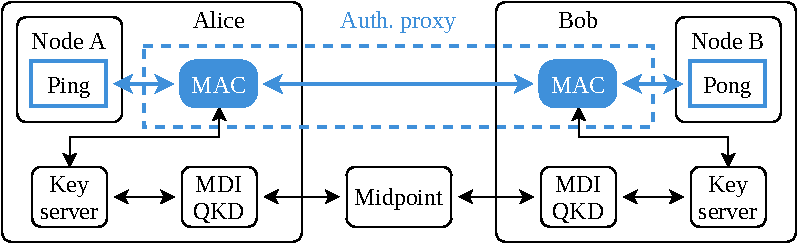
\includegraphics[width=0.6\linewidth]{figures/mac-setup-diagram.pdf}
    \caption{
        Experimental setup used to measure the end-to-end delays of transmitting an
        \emph{authenticated classical message} from Alice to Bob with \qty{42}{\km} of fiber-optic
        cables between them. Classical messages go through an authentication proxy that tags
        messages using \acrshort{mdiqkd}-generated key material.
    }
    \label{fig:mac-setup-diagram}
\end{figure}

\paragraph{Authentication proxy configuration}

We collect classical communication latency measurements under four different configurations of the
authentication proxy:

\begin{enumerate}
    \item Bypass proxy: at first, we bypass the authentication proxy altogether. This is useful to
          measure baseline communication latency, excluding all computation delays that would be
          introduced by the proxy.
    \item No \acrshort{mac}: this time, the proxy is configured to skip the authentication (and
          verification) step, but packets do go through the proxy's processing pipeline. Results for
          this configuration give us insights into the overhead of processing packets on the proxy,
          excluding the computation latency incurred by the \acrshort{mac} authentication (and
          verification) step.
    \item \acrshort{vmac}: in this configuration, the proxy computes and verifies message tags using
          the information-theoretically secure \acrshort{vmac} scheme~\cite{krovetz_2007_message}.
          We use both standard \acrshort{vmac} and a modified version that uses 21-bit tags
          (\acrshort{vmac}-21) instead of the default 64-bit tags.
    \item \acrshort{poly}: finally, we configure the proxy to use the computationally secure
          \acrshort{mac} called \acrshort{poly}~\cite{bernstein_2005_poly1305}. As opposed to
          \acrshort{vmac}, \acrshort{poly} can reuse the same key material for multiple messages.
\end{enumerate}

\paragraph{Rate and size of messages}

With the current implementation of the authentication proxy, one cannot transmit a classical message
more than once every \qty{10}{\ms} without experiencing detrimental packet loss. This contrasts with
the assumption in Ref.~\cite{dahlberg_2019_egp}, where \acrshort{mhp} messages are sent at a rate up
to \qty{100}{\kHz}. To circumvent this, we assume that \acrshort{mhp} messages may be batched
together and transmitted as part of a larger packet, and thus transmit ping messages at a rate of
\qty{100}{\Hz}.

Moreover, the current implementation of the proxy can only authenticate packets with a payload that
is small enough to be accommodated --- together with all protocol headers and the \acrshort{mac} tag
--- in a single Ethernet frame. Therefore, we send ping messages with payloads of
%
\begin{inlinelist}
    \item \num{12}~bytes, which is the size of the smallest \acrshort{qegp} message, and
    \item \num{1200}~bytes, which is close to the maximum allowed by the proxy.
\end{inlinelist}

\paragraph{Network topology}

The link connecting Alice to the center node runs for \qty{20}{\km}, whereas the link between Bob
and the center node is \qty{22}{\km} in length. Thus, the \acrshort{rtt} we measure is for a link of
a total length of \qty{42}{\km}. The topology of Alice, Bob, and the center node of the
\acrshort{mdiqkd} system is illustrated in \cref{fig:mac-setup-qkd-locations}.

\begin{figure}[t]
    \centering
    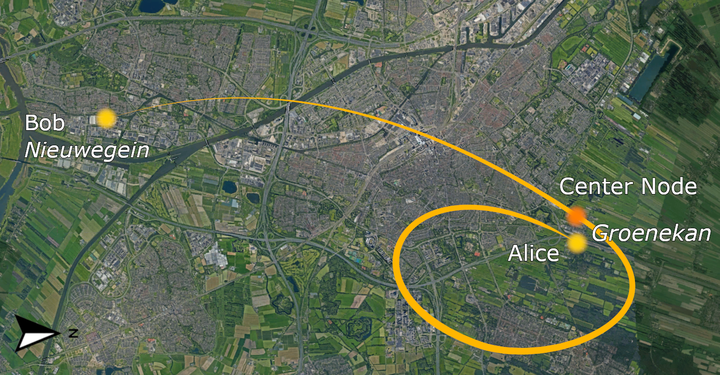
\includegraphics[width=0.6\linewidth]{figures/mac-setup-qkd-locations-resized.png}
    \caption{
        Physical layout of Alice and Bob nodes. Alice is located in Groenekan, the Netherlands,
        while Bob is in Nieuwegein, the Netherlands. The optical fiber connecting Alice to the
        center node is \qty{20}{\km} in length, whereas the connection between Bob and the center
        node is \qty{22}{\km}.
    }
    \label{fig:mac-setup-qkd-locations}
\end{figure}

\paragraph{Results}

We record the \acrlong{rtt} of \num{360000} ping messages per configuration (proxy configuration and
size of message). The computed mean and standard deviation of the results are reported in
\cref{tab:rtt}.

When bypassing the proxy altogether, the mean \acrshort{rtt} (less than \qty{4}{\ms}) is dominated
by propagation and transmission time through the experimental network. The small standard deviation
suggests that this baseline latency is quite stable. When messages go through the authentication
proxy but are not authenticated, the mean \acrshort{rtt} increases by a factor of around \num{3.5},
and the standard deviation becomes non-negligible. This is an indicator of the poor packet
processing performance of the proxy, which is merely a soft-processing packet pipeline implemented
in Python (the authentication proxy was designed for demonstration purposes, not performance). The
computational overhead introduced by the actual \acrshort{mac} is overshadowed by the baseline
latency of the proxy, as observed in the \acrshort{poly} configuration. Finally, statistics for the
\acrshort{vmac} configuration could not be computed at all, as far too many messages are dropped by
the proxy due to lack of key material. This is to be expected, given the high rate of key
consumption of the information-theoretically secure code. Interestingly, the size of messages does
not appear to be a noticeable factor in the mean end-to-end latency. We can therefore conclude that
latency is dominated by two main factors:
%
\begin{inlinelist}
    \item the length of the link, which depends on the network topology, and
    \item the packet processing performance of the proxy, which is approximately constant.
\end{inlinelist}

\section{Simulation Results}
\label{sec:doa:results}

We quantify the effects of using an authenticated classical channel for control messages exchanged
at the quantum network stack level. In particular, we augment the model used by
\textcite{dahlberg_2019_egp} to simulate the performance of physical (\acrshort{mhp}) and link
(\acrshort{qegp}) layer protocols within the quantum network stack. As opposed to the original work,
we model classical communication delays to also include transmission and authentication overhead,
when using \acrshort{poly} to authenticate messages, measured as described in
\cref{sec:doa:latency}. We report the \emph{throughput} of the quantum link, expressed as number of
entangled pairs generated per second.

\begin{table}
    \centering
    \begin{tabularx}{0.75\linewidth}{@{} lYYYY @{}}
        \toprule
        \textbf{Proxy}                     & \textbf{Tag size}          & \textbf{Payload} & \multicolumn{2}{c}{\textbf{\acrshort{rtt}} [\unit{\us}]}                 \\
        \cmidrule(l){4-5}
        \textbf{config}                    & [bits]                     & [Bytes]          & \textbf{mean}                                            & \textbf{std}  \\
        \midrule
        \multirow{2}{*}{Bypass proxy}      & \multirow{2}{*}{---}       & \num{12}         & \num{3656.61}                                            & \num{22.62}   \\
                                           &                            & \num{1200}       & \num{3881.37}                                            & \num{21.97}   \\
        \midrule
        \multirow{2}{*}{No \acrshort{mac}} & \multirow{2}{*}{---}       & \num{12}         & \num{13820.72}                                           & \num{3142.50} \\
                                           &                            & \num{1200}       & \num{13993.15}                                           & \num{2876.08} \\
        \midrule
        \multirow{2}{*}{\acrshort{poly}}   & \multirow{2}{*}{\num{128}} & \num{12}         & \num{14387.14}                                           & \num{5044.19} \\
                                           &                            & \num{1200}       & \num{13959.16}                                           & \num{2866.52} \\
        \midrule
        \acrshort{vmac}                    & any                        & any              & N/A                                                      & N/A           \\
        \bottomrule
    \end{tabularx}
    \caption{
        Mean and standard deviation of \acrfull{rtt} for different configurations of the proxy and
        for different message sizes. When using \acrshort{vmac}, most messages are dropped by the
        proxy due to lack of key material (resulting from the high rate of key consumption of
        \acrshort{vmac}), thus statistics are not available for that configuration.
    }
    \label{tab:rtt}
\end{table}

\paragraph{Configurations}

We run our simulations for two types of configurations:
%
\begin{inlinelist}
    \item To begin with, we study the performance of the link for several node-to-node distances, at
          a fixed requested fidelity ($F_\text{min}=0.65$). For the various distances, we scale the
          classical delays accordingly. For this configuration, we compare our augmented model with
          the original baseline, where transmission and authentication delays were not
          modeled~\cite{dahlberg_2019_egp}.
    \item Furthermore, we analyze quantum network throughput at a fixed node-to-node distance, but
          this time varying the requested fidelity at the \acrshort{qegp} layer. This time, we
          compare three models, corresponding to the three configurations of the proxy as per
          \cref{sec:doa:latency}: Bypass proxy, No \acrshort{mac}, and \acrshort{poly}. We do not
          report on \acrshort{vmac}, as we observed it requires more key material than our key
          server could supply (see \cref{sec:doa:latency}).
\end{inlinelist}

For each of the above configurations, we perform \num{20} simulation runs, each consisting of
\num{20} minutes of continuous use of the link. We then calculate the average throughput over all
runs for each configuration with a confidence interval of \qty{95}{\percent}.

\paragraph{Results}

\begin{figure}[t]
    \centering
    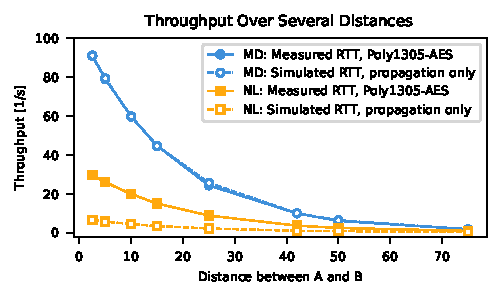
\includegraphics[width=0.6\linewidth]{figures/throughput_FCFS.pdf}
    \begin{tabularx}{0.6\linewidth}{@{} lYYYYYYYY @{}}
        \toprule%
                        & \multicolumn{8}{c}{\textbf{Breakdown of distance A -- B [\unit{\km}]}} \\%
        \midrule%
        \textbf{A -- M} & 1.5 & 3 & 6  & 9  & 15 & 22 & 30 & 45 \\%
        \textbf{M -- B} & 1   & 2 & 4  & 6  & 10 & 20 & 20 & 30 \\%
        \midrule%
        \textbf{Total}  & 2.5 & 5 & 10 & 15 & 25 & 42 & 50 & 75 \\%
        \bottomrule%
    \end{tabularx}%
    \caption{
        Throughput (rate) of entangled pair generation for multiple distances between node A and B,
        with a single midpoint station in between and for a requested fidelity of
        $F_\text{min}=0.65$. Classical communication delays were modeled using latency measurements
        collected as described in \cref{sec:doa:latency} (configuration ``\acrshort{poly}''), as
        well as replicated from the original simulations of \acrshort{qegp} and
        \acrshort{mhp}~\cite{dahlberg_2019_egp}. The table shows how distance is distributed between
        A, B, and the midpoint station. The \qty{25}{\km} data point is equivalent to the QL2020
        hypothetical setup simulated in Ref.~\cite{dahlberg_2019_egp}. The solid line represents
        mean throughput, the colored area around it depicts the \qty{95}{\percent} confidence
        interval.
    }
    \label{fig:results-distance}
\end{figure}

The results for throughput versus distance are illustrated in \cref{fig:results-distance}. For
\acrfull{md} type requests, mean throughput is approximately equal across the two models of
classical delays. This is to be expected, given that these types of requests can be pipelined, and
thus throughput is mostly dominated by the physical entanglement generation procedure, not as much
by classical communication latency. On the other hand, \acrfull{nl} requests --- which, for our
purpose, are equivalent to \acrfull{ck} requests --- show a more surprising outcome: the throughput
is higher for the configuration where classical communication models transmission authentication
delays on top of the propagation delays from the baseline~\cite{dahlberg_2019_egp}. We attribute
this effect to the fact that when classical communication is faster, \acrshort{qegp} request are
distributed at a faster rate, and thus the request queues fill up more quickly, resulting in a
higher request rejection rate. The discrepancy between our model and the baseline is especially
clear at shorter distances, where classical communication in the baseline model is considerably
faster than in our model.

The results for throughput versus fidelity are shown in \cref{fig:results-fidelity}. For this
experiment, the outcome just matches our expectations. \acrshort{md} requests are not affected by
classical communication much, and their throughput only decreases when higher-fidelity entangled
pairs are requested. \acrshort{nl} requests, instead, are more affected by classical communication
latency, and their throughput decreases more noticeably when classical messages go through the
authentication proxy. As expected from the results in \cref{tab:rtt}, the extra delays incurred by
the actual \acrshort{mac} computation are negligible, and their effect on throughput not noticeable.

\section{Discussion}

We have shown how the classical data plane of the quantum network stack presents a significant
attack surface for \acrlong{cia} of the quantum link and data. To address these concerns on must
employ, among other things, \acrlong{doa} on the classical control messages exchanged at the quantum
network stack level. We conclude that \acrlong{doa} is necessary to both uphold the integrity of
quantum data and the availability of the quantum network itself.

\begin{figure}[t]
    \centering
    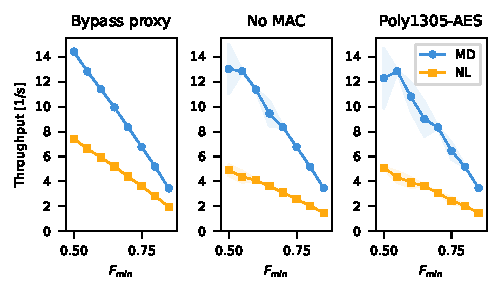
\includegraphics[width=0.6\linewidth]{figures/throughput_FCFS_mhp_150.pdf}
    \caption{
        Throughput (rate) of entangled pair generation for multiple requested fidelities, with
        \qty{20}{\km} between node A and the midpoint station, and \qty{22}{\km} between the
        midpoint station and node B, and for three configurations of the proxy as per
        \cref{sec:doa:latency}: Bypass proxy, No \acrshort{mac}, and \acrshort{poly}. \acrshort{vmac}
        results are omitted as packet drop rates are excessive. The solid line represents mean
        throughput, the colored area around it depicts the \qty{95}{\percent} confidence interval.
        \Acrfull{md} type requests are not as heavily affected as these are pipelined. \Acrfull{nl}
        type requests are performed sequentially, and thus increases in classical delays have a more
        profound impact on throughput.
    }
    \label{fig:results-fidelity}
\end{figure}

We have also simulated the performance of a hypothetical quantum link under the assumption that
classical messages were being authenticated in some sort of way. Here, we modeled classical
communication latency, including authentication overhead and transmission delay, using metrics
collected from a classical link authenticated using key material sourced from an \acrshort{mdiqkd}
system. If we disregard the large packet processing delays incurred by the authentication proxy used
in this work, we observe that an authenticated classical channel introduces a negligible amount of
extra classical overhead, provided that one uses an optimized \acrshort{mac}.

However, we have also seen that propagation and transmission delays themselves have a noticeably
negative effect on the performance of a quantum link, whether or not \acrlong{doa} is applied. While
the quantum link remains functional, the entanglement generation rate drops by a significant amount
for entanglement requests that do not end with an immediate measurement of the entangled qubit.

\printbibliography[heading=subbibintoc,title={References},notcategory=noprint]
